\begin{align*}
f(x)=\left\{\begin{array}{ll}
h(x)&\mbox{ für }1\le  x\le x_0\\
af(\frac{x}{b})+g(x)&\mbox{ für }x>x_0
\end{array}\right.
\end{align*}
\fbox{\parbox{\columnwidth}{Verallgemeinerte Form:
\begin{align*}
\sum_{i=1}^m a_if\left(\frac{x}{b_i}\right)+g(nx)\,\mbox{ für }\, x>x_0
\end{align*}
}}\\[.5em]
\[a>0,b>1,g:\mathbb R^+\rightarrow\mathbb R^+\]
\small
\begin{align*}
&\exists d_1,d_2>0: d_1\le h(x)\le d_2\mbox{ für }1\le x\le x_0\\
&\exists c_1,c_2>0:c_1g(x)\le g(u)\le c_2g(x)\mbox{ für }x-\frac{x}{b}\le u \le x 
\end{align*}
\normalsize
\[f(x)\in\theta(x^p(1+\int_1^x\frac{g(u)}{u^{p+1}}du))\]
mit $p=\log_ba,b^p=a$\\
Beweis (Idee):
\begin{align*}
f(x)&=af(\frac{x}{b})+g(x)\\
f(\frac{x}{b}&=af(\frac{x}{b^2})+g(\frac{x}{b})\\
&\vdots\\
f(x)&=a^kf(\frac{x}{b^k}+\sum_{i=0}^{k-1}a^ig(\frac{x}{b^i})\\
\end{align*}
bis $\frac{x}{b^k}=1\Rightarrow k=\log_bx$\\[.5em]
\fbox{\parbox{\columnwidth}{Beispiel:
\[H_n=\sum_{i=1}^n\frac{1}{i}\approx \int_1^n\frac{1}{x}dx\approx\ln n\]
\center
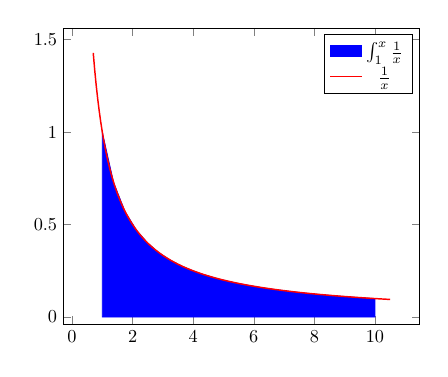
\begin{tikzpicture}[scale=0.66]
\begin{axis}[legend entries={$\int_1^x\frac{1}{x}$,$\frac{1}{x}$}]
\addplot+[area legend,no markers,fill=blue,domain=1:10]{1/x} \closedcycle;
\addplot+[no markers,thick,domain=0.7:10.5,samples=200]{1/x};
\end{axis}
\end{tikzpicture}
}}
\[\sum_{i=0}^{k-1}a^ig(\frac{x}{b^i})\approx \int_0^{k-1}a^ig(\frac{x}{b^i})di\]
\fbox{\parbox{\columnwidth}{Substitution:
\begin{align*}
u&=\frac{x}{b^i}=cb^{-i}\\
\frac{du}{di}&=-\ln b x b^{-i}\\&=-\ln b u\\
di&=-\frac{1}{\ln b u}du
\end{align*}
}}\\[.5em]
\begin{align*}
\Rightarrow\,&=-\frac{1}{\ln b}\int a^ig(u)\frac{1}{u}du\\
&=\frac{1}{\ln b}\int_b^x(\frac{x}{u})^pg(u)\frac{1}{u}du\\
&=\frac{1x^p}{\ln b}\int_b^x\frac{g(u)}{u^{p+1}}du
\end{align*}
mit
\begin{align*}
&i=\log_b\frac{x}{u}\\
&a^i=b^{\log_ba\log_b\frac{x}{u}}=(\frac{x}{u})^{\log_ba}=(\frac{x}{u})^p\\
&i=k-1\Rightarrow u=xb^{-k+1}=(\frac{x}{b^k})b
\end{align*}

\subsection{Anwendung von Akra Bazzi}
$$T(n)=2T(\frac{n}{2})+n\log n$$
$$g(n)=n\log n$$
$$T(n)=\theta (n^1(1+\int_1^n\frac{u\log u}{u^2}du))$$
$$p=\log_ba=1$$
$$\int_1^n\frac{\ln u}{u}du=[\ln^2u]_1^n=\frac{1}{2}\ln^2n$$
$$T(n)=\theta(n(1+\log^2n))=\theta(n\log^2n)$$